%%
%% This is file `mcmthesis-demo.tex',
%% generated with the docstrip utility.
%%
%% The original source files were:
%%
%% mcmthesis.dtx  (with options: `demo')
%%
%% -----------------------------------
%%
%% This is a generated file.
%%
%% Copyright (C)
%%     2010 -- 2015 by Zhaoli Wang
%%     2014 -- 2016 by Liam Huang
%%
%% This work may be distributed and/or modified under the
%% conditions of the LaTeX Project Public License, either version 1.3
%% of this license or (at your option) any later version.
%% The latest version of this license is in
%%   http://www.latex-project.org/lppl.txt
%% and version 1.3 or later is part of all distributions of LaTeX
%% version 2005/12/01 or later.
%%
%% This work has the LPPL maintenance status `maintained'.
%%
%% The Current Maintainer of this work is Liam Huang.
%%
\documentclass{mcmthesis}
\mcmsetup{CTeX = false,   % 使用 CTeX 套装时,设置为 true
        tcn = 2014906, problem = A,
        sheet = true, titleinsheet = true, keywordsinsheet = true,
        titlepage = true}
\usepackage{palatino}
\usepackage{mwe}
\usepackage{graphicx}
\usepackage{subcaption}
\usepackage{float}
\usepackage{multirow}
\usepackage{indentfirst}
\usepackage{gensymb}
\usepackage[ruled,lined,commentsnumbered]{algorithm2e}
\usepackage{geometry}

%% ADDED
\usepackage{mathtools}
\usepackage{setspace}



\begin{document}
\linespread{0.6} %%行间距
\setlength{\parskip}{0.5\baselineskip} %%段间距

\title{Novel Coronavirus Pneumonia: Aloha and to Say Aloha}

\date{\today}
	\begin{abstract}
\hspace{1.2em}
	Begin Abstract...
		\begin{keywords}
			Begin Keywords...
		\end{keywords}
	\end{abstract}


\maketitle

\tableofcontents

\newpage


\section{Introduction}	\label{S1}

\subsection{Problem Background}
	The ocean is covering approximately 1.3 billion cubic kilometers on Earth, which is the equivalent of 97 percent of total water. Playing a vital role in oxygen producing, carbon sequestering and food providing for billions of people, the ocean's abilities are being eroded by plenty of stressors. \par
	Since the 1950s, the oceans hava absorbed more than 93 percent of all the heat that produced by human, which is beginning to show its drawbacks at a price. Marine organisms, as an import part in the ocean, can be affected when there are changes in their natural habitat as well as changes in ocean chemistry. As a primary producer of the food chain in the ocean, phytoplankton, a kind of marine plants, is facing a incrementally decrease if the water becomes warmer, which results in the reduction of the amount of nutrients in the ocean. The scarcity of nutrients will limit the growth of marine organisms in the food chain. In addition, temperature plays an important role in controlling biological rhythm of marine plants and animals involving birth, growth, feeding, production and death. The changes in ocean temperature will cause a disruption of biological rhythm making marine organisms become vulnerable to illness. Moreover, sequence lowering of the pH of seawater is unfavorable to the hatching of eggs and the growth of fry of some sea fish.\par
	The anticipated increase in ocean temperature is predicted to stimulate the migration of marine organisms based on their temperature tolerance, with heat-tolerant species expanding their range northward and those less tolerant species retreating. Just as the lobster of Maine, USA, thousands of aquatic species is forced to migrating north to find a better habitat. As an impact, relative companies need to move their base to survive. \par
	

\subsection{Our Work}
	Based on our understanding of the problem, we make Gray Prediction Model as well as Differential Equations to predict the location of fish. Sequenced analysis are based on our prediction.\par
	The remainder of this article is organized as follows. In Section \ref{S2} and Section \ref{S3}, we put forward
main assumptions and notations in this paper. Section \ref{S4} shows our predicting process. Section \ref{S5} ... .In Section \ref{S6}, ... . In Section \ref{S7}, we discuss the strengths
and weaknesses of our models. And finally, we conclude the paper in Section \ref{S8}.
	The major logic flow is depicted as follows, in Figure \ref{fig:flow}:
	
	\begin{figure}[H]
    \centering
    \includegraphics[width=1\textwidth]{plots/flow_V1.jpg} %%% \textwidth 可以改图片大小
    \caption{Major Logic Flow of our Model - ALOHA}
    \label{fig:flow}
    \end{figure}
    %% Flow Chart %%%


\section{Assumptions and Justifications}\label{S2}
    We make some general assumptions to simplify our model. We will list some general assumptions with corresponding justification below:
\begin{enumerate}[1)]
	\item\label{ass1} {\bfseries Fishes will move towards the position where the living condition is suitable for them.} Most fish prefer to live in warmer places than in colder ones. As the temperature changes, the fish changes range of activity to a zone of water suitable for its existence.
	\item\label{ass2} {\bfseries Sea surface temperature is the determinant leading to the migration of fishes.} This assumption is directly from Assumption \ref{ass1}. As the temperature in different depth in the ocean is distinct, which is affected by many factors making it hard to predict, we just assume the temperature in different depth is the same as the surface temperature.
	\item\label{ass3} {\bfseries Fish will not change living habits in the next fifty years.} It usually takes thousands of years for species to adapt to the living environment. Once living habit is established, it is hard to change. Fifty years is a short period of time, the change of living habits can be ignored. 
	\item\label{ass4} {\bfseries Fishing companies always pursue maximum profit.} A company is in need of making profit to survive and expand. We regard making profit as the first law for corporation to survival. That is to say, decisions are made for sake of maximized profit.
	\item\label{ass5} {\bfseries The fish schools are around four major ports in Scotland.} With abundant fish schools, these company can always expand their industries. Thus, we assume that main fish schools are around the major companies in Scotland.
\end{enumerate}


\section{Notations and Definitions}\label{S3}
    For convenience, we define a series of notations for mathematical usage, which are listed in Table \ref{notation} to describe our model.
\begin{table}[H]\normalsize
    \centering
    \caption{Notations mentioned in this paper}
    \label{notation}
    \begin{tabular}{c c}
\toprule[2pt]
        Symbol & Definition\\
\hline
    $S(t)$ & Number of susceptible person at time t\\
    $E(t)$ & Number of enfective person at time t\\
    $I(t)$ & Number of infectious person at time t\\
    $R(t)$ & Number of removed person at time t\\
    $t$ & Time\\
    $N$ & Gross population in this model\\
    $\alpha$ & Morbidity of NCP\\
    $\beta$ & Infection rate\\
    $\gamma$ & Removal rate\\
    $d$ & Mortality of NCP\\
    $h$ & Recovery rate of NCP\\
    $k$ & Average number of people exposed to infections every day \\
    $b$ & Probability of infection by contact\\
    $R_0$ & Basic reproduction number\\
    $m_i$ & Affecting parameters of $ith$ measure by government \\
    $ND$ & Number of death\\
    $NR$ & Number of recovery\\
    $NSP$ & Number of suspected people\\
    $NDP$ & Number of diagnosed people\\
\bottomrule[2pt]
    \end{tabular}
\end{table}



\section{Model Analysis} \label{S4}
		In this section, we present the \textbf{Gray Forecasting} method to simulate the change of the average sea surface temperature of a region on the ocean. Also, we use \textbf{Differential Equation} to introduce the influence of global warming to the temperature. The framework of the model is shown in Figure 1. Referencing the temperature data onto recent years, we calculate the factors of our model using Gray Forecasting, which can identify the degree of variation in development trends among system factors. After conducting the solution by Gray Forecasting, we additional add the global warming factor of the heavier of carbon emission. Finally, we analyze the immigration of these two fish species as well as the most likely location for these two fish species over the next 50 years.
	% ADD Flow Chart of Model 1

\subsection{Sea Surface Temperature Forecasting Model}\label{S4s1}
	The temperature on the ocean always gets affected by a huge number of factors, including solar radiation, ocean currents, carbon emission, El Nino phenomenon, etc. To avoid the complex analysis and simplify the problem, we use a gray forecasting model to calculate the correlation degree of factors. Besides, the acceleration of global warming, extra differential equations are needed as correction of our model.

\subsubsection{SST Based on Gray Forecasting}\label{S4ss1}
	We first denote the symbols and terms used in this part.
\begin{table}[H]\small
    \centering
    \caption{Symbols and Terms}
    \label{symbol}
    \begin{tabular}{c c}
\toprule[2pt]
        Symbol & Definition\\
\hline
    $SST$ & Sea surface Temperature \\
    $AGO$ & Accumulated Generating Operation\\
    $GM(1,1)$ & Gray Model\\
    $IAGO$ & Inverse Accumulated Generating Operation\\
    $...$ & ...\\
\bottomrule[2pt]
    \end{tabular}
\end{table}
	According to the already existing SST data\cite{sstdata}, we initialize our forecasting model using monthly statistics from January, 2006 as the first month to January, 2020 .\par
	Assuming that the SST in the original k-th month is $x^{(0)}(k)$, set the original data as follows:
\begin{equation*}
	x^{(0)} = x^{(0)}(1), x^{(0)}(2), ..., x^{(0)}(n)
\end{equation*}\par
	We denote
\begin{equation*}
	x^{(1)}(k) =  \sum_{i=1}^kx^{(0)}(i) \qquad  ,where\quad k = 1, 2, ..., n
\end{equation*}\par
	Then, we calculate the class ratio $\lambda{k}$
\begin{equation*}
	\lambda(k) =  \frac{x^{(0)}(k-1)}{x^{(0)}(k)}
\end{equation*}\par
	Due to all $\lambda k \in \big[0.982, 1.0098\big]$, we can reach a satisfying model using GM(1,1).
	By $AGO$, 
\begin{equation*}
	x^{(1)}(k) =  \sum_{i=1}^kx^{(0)}(i) \qquad  ,where\quad k = 1, 2, ..., n
\end{equation*}\par
	Take differential, i.e.
\begin{equation*}
	d(k) = x^{(0)}(k) = x^{(1)}(k) - x^{(1)}(k-1)
\end{equation*}\par
	Denote $z^{(1)}(k)$ as the adjacent value generated sequence, i.e.
\begin{equation*}
	z^{(1)}(k) = \alpha x^{(1)}(k) + (1-\alpha)x^{(1)}(k-1)
\end{equation*}\par
	So, we get the model as
\begin{equation*}
	d(k) = \alpha z^{(1)}(k) = b
\end{equation*}\par
	We then construct Data Matrix $B$ and Data Vector $Y$
\begin{equation}
	B =  \left[ \begin{matrix}
						-\frac{1}{2}(x^{(1)}(1)+x^{(1)}(2))  & 1 \\
						-\frac{1}{2}(x^{(1)}(2)+x^{(1)}(3))  & 1 \\
										...									& ... \\
						-\frac{1}{2}(x^{(1)}(k)+x^{(1)}(k+1))  & 1 \\
\end{matrix}\right],
	Y =  \left[ \begin{matrix}
						x^{(0)}(2)\\
						x^{(0)}(3)\\
							...    \\
						x^{(0)}(k)\\
\end{matrix}\right]
\end{equation}\par
\begin{equation*} 
	\hat{\mu} = (a, b)^{T} = (B^{T}B)^{-1}B^{T}Y = (3.21*10^{-4},295)^{T}
\end{equation*}\par
\begin{equation*}
	\frac{dx^{(1)}}{dt} + 3.21*10^{-4} x^{(1)} = 295
\end{equation*}\par
	Solution is, 
\begin{equation*}
	x^{(1)}(k+1) = (x^{(1)}(k) - \frac{b}{a})e^{-ak} + \frac{b}{a} 
\end{equation*}\par
	Until now, we get the forecasting value of future sea surface temperature. \par
	Rechecking: \par
	We compared the results obtained by this model with the true situation from 2006 to 2020, conducting the residual relative to the actual data. The following figure shows the residual distribution, from which we can tell the accuracy of our prediction.\par
     \begin{figure}[H]
     \begin{minipage}{0.5\linewidth}
       \centerline{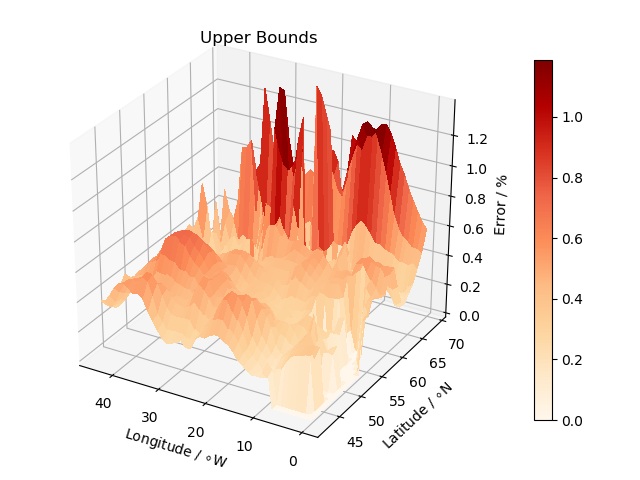
\includegraphics[width=9.0cm]{plots/grey_forcast_err_1_V1.png}}
       \centerline{(a) Upper Bounds}
     \end{minipage}
     \hfill
     \begin{minipage}{.5\linewidth}
       \centerline{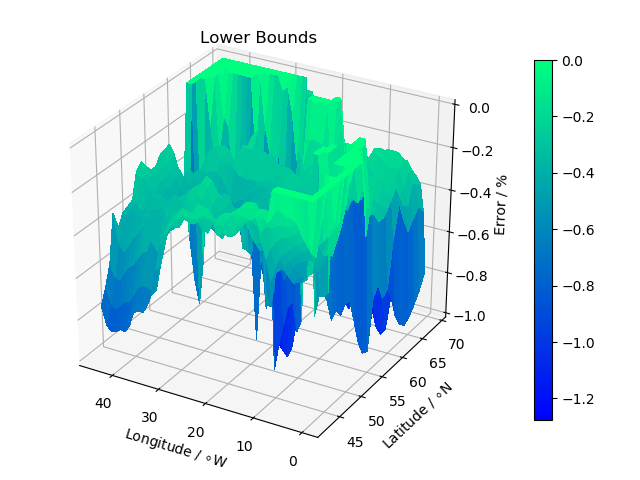
\includegraphics[width=9.0cm]{plots/grey_forcast_err_2_V1.png}}
       \centerline{(b) Lower Bounds}
     \end{minipage}
     \caption{Residual Distribution}
     \label{figures}
     \end{figure}

\subsubsection{Influence of Global Warming}\label{S4ss2}
	Equation \ref{set1} shows the mathematical foundation of the influence of global warming. The parameters are defined as follows:

\begin{itemize}
	\item $\rho$ indicate the density of the ocean. Since there are only delicate distinction between different region, we let $\rho$ approximately equal to 1. 
	\item \emph{h} shows the mixed layer depth, which we take\cite{globalwarming}
		\begin{equation*}
		\emph{h}  = 70m \cite{globalwarming}
		\end {equation*}
	\item $C_p$ shows the specific heat of a part of ocean, which is assumed as $60000000J$.
	\item $\gamma$ is a parameter defined in terms of the fraction of land. We assume $\gamma \in \big[0.72,0.75\big]$ \cite{co2dat}
	\item $\lambda$ the climatic feedback factor, which is defined as \cite{globalwarming}
		\begin{equation*}
		\lambda = 3.58 W m^{-2} K^{-1}
		\end {equation*}
	\item  $\delta F$ express the flux lost from the mixed layer, which is ignored in our model. 
	\item $\Delta Q$ shows the net surface flux, which is defined as\cite{modelsol}
		\begin{equation*}
		\delta Q = 34.6534 \times 10^{-4}te^{8.686\times 10^{-3}t}
		\end {equation*}
	\item \emph{t} indicates the number of the year, such as 2018, 2019, etc.
\end{itemize}
\par
	After acquiring these parameters, we can establish a Box-Diffusion Model\cite{funct} to predict temperature change sequenced by carbon dioxide emission in the next fifty years. Differential equation \ref{set1} represents the relationship between sea surface temperature and time. It is already know that the interaction between carbon dioxide and sea happens in the mixed layer. Therefore, $\Delta Q$ can be used as a measuring standard of carbon dioxide. The main cause of global warming in recent decades is the exacerbated greenhouse effect resulting from the increasing emission of carbon. To illustrate the relation of global warming and sea surface temperature, we establish Differential Equation \ref{set1}.
\begin{spacing}{1.5}
\begin{equation*}\label{set1}
\gamma\rho C_{p} h\frac{d\Delta T}{dt} = \Delta Q - \lambda\Delta T - \Delta F
\end{equation*}
\end{spacing}
\par
	We make use of computer program to solve the differential equation. However, the numerical solution we get is discrete, we have to use the fitting method to simulate the changing situation. We find the relationship between temperature and time is linear, which means the average sea surface temperature will rise at a constant speed under the influence of global warming. By our prediction, the sea surface temperature will rise about 0.033 Centigrade each year. The fitting result is shown below.
%picture here 
\par

\subsection{FISH: Fish Immigration Simulation Heuristic Model}\label{S4s2}
	Based on the water temperature predictions we finished in Section \ref{S4s1}, we can get the main position where these two fish species located in the next 50 years by \textbf{FISH Model}. In section \ref{S4s21}, we arrange some simplifications and corresponding justification to illustrate. In section \ref{S4s22}, we give further details and results as well as sequenced analysis based on the model.\par
	
\subsubsection{Simplification and Justification}\label{S4s21}
	In order to simplify our model, we make the following assumptions:
\begin{enumerate}[1)]
	\item {\bfseries A school of fish will not scatter during immigration.} The randomness of scattering will profoundly increase the difficulty. Accordingly, we ignore the case of scattering in this paper.
    \item {\bfseries The sea surface temperature can represent the temperature at which fishes live.} This assumption is just a specification of Assumption \ref{ass2}. Since the ocean is too deep for us to analyze the temperature in different depth, we simply take the surface temperature to present the temperature where fishes live.
% 	\item {\bfseries Fish will move towards the suitable position.} According to biological theory, animals tend to move to the suitable place to live if their current habitat is not suitable.
\end{enumerate}	\par
     % 两种鱼的相似性 
    Another reasonable simplification is that \textbf{we consider herring and mackerel as similar species}. This is supported by many arguments. We list several of them in the following list:
\begin{itemize}
	\item Herring and mackerel are similar in their length and weight as well as the capability of swimming. According to documentation, herring is always  about $40cm$, one kilometer, while mackerel is just a bit heavier than herring. Also, they both can swim in a quick speed, which shows they enjoy the same level of mobility\cite{Wiki_herring}\cite{Wiki_mackerel}.
	\item In terms of trophic level, they both prey on phytoplankton as well as small crustaceans such as copepods, forage fish, shrimp, and squid. There are not significant differ in their positions in food chain.
	\item They both live in mid-water pelagic environments\cite{Wiki_herring}\cite{Wiki_mackerel}. The similar living condition of herring and mackerel allows them living under similar temperatures under ocean. 
	\item Herring and mackerel are fished for by similar ships. As is claimed by Scottish Government, herring and mackerel are mainly targeted by the pelagic fleet, which always has large, profitable vessels\cite{scotmarine}. 
\end{itemize}
\subsubsection{FISH Model and Results}\label{S4s22}
	 Due to the initial place of fish school is unknowable, we choose four major fishing ports as the most possible region as the starting region. To iterate, we decide to choose eight directions as the moving directions. Each iteration contains a movement towards one certain direction where the temperature is favorable to the fish school. The algorithm that we use in FISH Model is shown as Algorithm \ref{alg1}.\par


\IncMargin{1em}
\begin{algorithm}[H]
\SetKwData{SST}{SST}
\SetKwData{y}{year}
\SetKwData{l}{sea}
\SetKwData{d}{direction}
\SetKwInOut{Input}{input}\SetKwInOut{Output}{output}

\Input{Fish's Starting Position (X, Y), Predicted Yearly Temperature Data }
\Output{Fish's Positions in the next 50 Years}
\BlankLine
\BlankLine
\emph{Initialize fish school starting position $ (x, y) = (X, Y)$}\;
\SetAlgoLined\SetArgSty{}
\For{$\y$ $\leftarrow$ 0 $\KwTo$ 50}{
\emph{Generating Moore Neighborhood of (x, y): MH(x, y)}\;
\For{$\d \in MH(x, y) = \left[NW, W, SW, S, SE, E, NE, N\right]$}{
    \If{$(x_{i},y_{i})$ is $\l$} {
	$\sigma_i = \left \|\SST(x_i, y_i, \y+1) - \SST(x,y,\y)\right \|$}}
    find $i_{min}$, $\quad$ s.t. $\sigma_{i_{min}} \leq \sigma_i$ ,for $\forall i$ \;
\If{$\sigma_{i_{min}} < \delta $} {  
$(x, y) \leftarrow (x_i, y_i)$}
}
\caption{Fish Immigration Simulation Heuristics}\label{alg1}
\end{algorithm}\DecMargin{1em}\par
    According to Assumption \ref{ass5}, we take several locations of fishing ports as just the positions where fishes live. The port locations we choose are listed in Table \ref{loca}. Starting from the initial longitude and latitude coordinate, fishes would always move to the next coordinate with the closest temperature. The sea surface temperature prediction model we built in section \ref{S4s1} provides temperature data yearly. Thus, here we also calculate forty-nine times' movement of fish schools in the next fifty years. Each time the fish schools' movement leads to one degree's change in either longitude or latitude or together. It is worth mentioning that if the temperatures of  eight directions are all different from the central coordinate ``a lot", the fish will stay at the same position till the next year. Exactly, we set the maximum of difference to be 0.5 Centigrade as a measuring standard of ``a lot". In short, if the differences between central position's temperature and eight surrounding positions' temperatures are all greater than 0.5 Centigrade, the fishes will not move in this year. In Algorithm \ref{alg1}, symbol $\delta$ means the allowed temperature difference 0.5 Centigrade. \par
\begin{table}[H]\normalsize
    \centering
    \caption{Fishing Ports Information Table}
    \label{loca}
    \begin{tabular}{c c c}
\toprule[2pt]
        Fishing Port & Latitude & Longitude\\
\hline
    Stornoway & 57.7N & 2.03W\\
    Ayr & 55.5N & 4.63W\\
    Campbeltown & 55.5N & 5.54W\\
    Ullapool & 57.9N & 2.51W\\
    Portree & 57.4N & 6.2W\\
\bottomrule[2pt]
    \end{tabular}
\end{table}
    \par
	We input the longitude and latitude coordinates of the chosen fishing ports shown in Table \ref{loca}. After 50 rounds of iteration, a solution figure can easily get. Such solution figure shows the  result of fish immigration simulation. The detailed information is shown in the Figurelalalalalala \par % 这里加入图片



\subsection{Analysis for Small Fishing Companies}\label{S4s3}
	From previous models, we predict the position of fish schools in the next 50 years. In terms of small fishing companies, whose ability to make distant voyage is relatively low, the location of fish school will definitely determine their destiny. Our team, in this section, arrange some method to evaluate the different cases that may occur in the next 50 years according to the immigration processes of fish schools.\par
	    % 算法简介 Here
	    
	    % 步骤解释 这里
	    
	    % 结果分析 这里
	    
\section{title}\label{S5}

\subsection{Background Illustration}
   
    
\subsection{subsection1}\label{S5s1}
    

\subsection{subsection2}\label{S5s2}
	
 
\section{S6}\label{S6}
   
	
\subsection{Simulation Results}
    


\section{Model Analysis}\label{S7}

\subsection{Sensitivity Analysis}


\subsection{Strengths and Weaknesses}
\subsubsection{Strengths}
\begin{itemize}
	\item Our model achieves a good simulation in fitting the current infections.
	\item Our model takes into account the effects of the change of pedestrian flow during the Spring Festival travel rush as well as virus mutations
	\item The model is a well-organized epidemic model which can be widely applied to other virus disease.
\end{itemize}
\subsubsection{Weaknesses}
\begin{itemize}
	\item The prediction simulation result can't be verified due to the unknown data in future.  
	\item A large number of assumptions reduce the accuracy of the model’s simulation results.
\end{itemize}


\section{Conclusion}\label{S8}


\newpage


\bibliographystyle{IEEEtran}
\bibliography{newrefs}

\section*{Brief Assessment Report}\label{S9}

\newpage

\begin{appendices}

\section{Solve and Plot Ordinary Differential Equation Systems}
\lstinputlisting[language=Python]{ODES.py}

\end{appendices}


\newpage


% \section{Figures}

% %%  单图片模型(不要复制这句话)
% 	\begin{figure}[H]
%     \centering
%     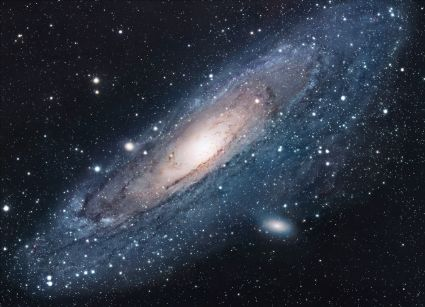
\includegraphics[width=0.7\textwidth]{universe.jpg}%%% \textwidth 可以改图片大小
%     \caption{biao ti ?}
%     \label{Fig_1}
%     \end{figure}
%     %%% 需要的话,请在这里写图片说明,否则不要复制 %%%
    
% %% 1*n图片模型(不要复制这句话)
%     \begin{figure}[htbp]
%         \begin{minipage}[t]{0.45\linewidth}
%         \centering
%         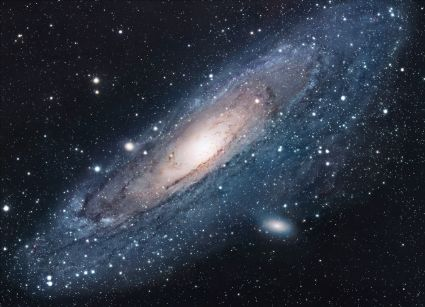
\includegraphics[height=4cm,width=4cm]{universe.jpg}
%         \caption{cite??}
%         \end{minipage}%
%         \begin{minipage}[t]{0.45\linewidth}
%         \centering
%         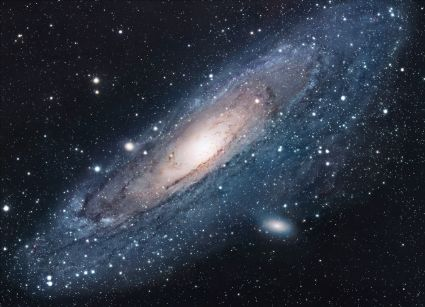
\includegraphics[heThis is the usage\cite{Wiki_bathtub,mankiw2014principles,finite} of Latex\cite{finite}.
	
% ight=4cm,width=4cm]{universe.jpg}
%         \caption{biao ti ?}
%         \end{minipage}
%     \end{figure}
%      %%% 需要的话,请在这里写图片说明,否则不要复制 %%%
    
% %% 合并图片(不要复制这句话)
%     \begin{figure}
%     \begin{minipage}{0.48\linewidth}
%       \centerline{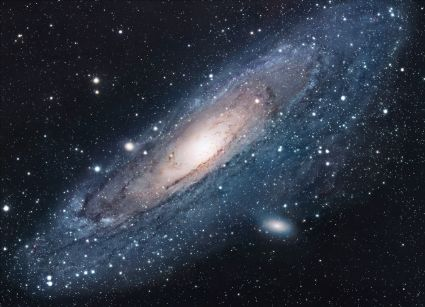
\includegraphics[width=4.0cm]{universe.jpg}}
%       \centerline{(a) Result 1}
%     \end{minipage}
%     \hfill
%     \begin{minipage}{.48\linewidth}
%       \centerline{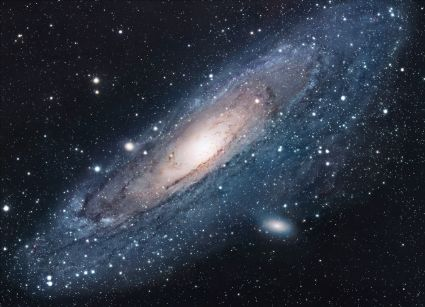
\includegraphics[width=4.0cm]{universe.jpg}}
%       \centerline{(b) Results 2}
%     \end{minipage}
%     %% 如果需要 多纵列的话
%     \vfill
%     \begin{minipage}{0.48\linewidth}
%       \centerline{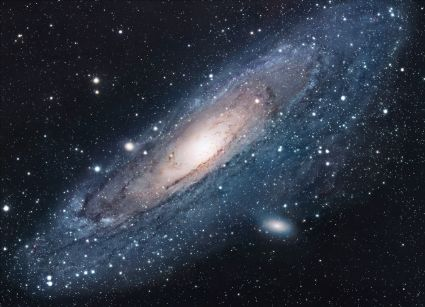
\includegraphics[width=4.0cm]{universe.jpg}}
%       \centerline{(c) Result 3}
%     \end{minipage}
%     \hfill
%     \begin{minipage}{0.48\linewidth}
%       \centerline{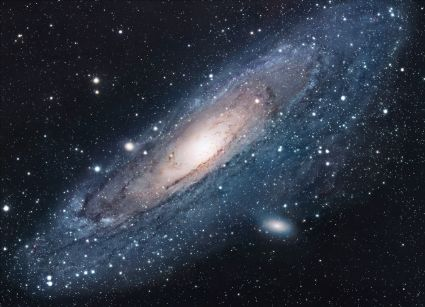
\includegraphics[width=4.0cm]{universe.jpg}}
%       \centerline{(d) Result 4}
%     \end{minipage}
%     %\end{tabular}
%     \caption{Examples of aaa}
%     \label{figures}
%     \end{figure}

%%%%%%%%%%%%%%%%%%%%%%%%%%%%%%%%%%%%%%%%%%%%%%%%%%%%%%%%%%%%%%%%%%%%%%%



\end{document}

%%
%% This work consists of these files mcmthesis.dtx,
%%                                   figures/ and
%%                                   code/,
%% and the derived files             mcmthesis.cls,
%%                                   mcmthesis-demo.tex,
%%                                   README,
%%                                   LICENSE,
%%                                   mcmthesis.pdf and
%%                                   mcmthesis-demo.pdf.
%%
%% End of file `mcmthesis-demo.tex'.
